\section{Defending against compression attacks}\label{sec:defense}
Keeping in mind our theoretical model, we determine the key elements that make these
attacks possible.

We propose a defense, \textit{context hiding}, that mitigates a class of
practical compression side-channel attacks such as CRIME, TIME, BREACH, Rupture,
and HEIST. The full plaintext recovery these attacks perform is no longer
possible when our defense is applied.

\subsection{Hardness of defending}
First of all, observe that there is a trivial method of defense, and that is
disabling compression completely.

However, defending against an adversary by modifying $f$ is hard in general. We
note that $f$ is required to be polynomially reversible, meaning it must contain
enough information to recover $s$. Because $Com$ must be able to decrease the
length of various plaintexts, it can output plaintexts of different lengths
dependent on $s$. Therefore, if $Com$ is adversarial, it can easily leak
information through the encryption function $Enc$ by using its output length. As
such, any attempt to generally defend against all compression functions $Com$ is
necessarily futile.

However, the fact that it is theoretically difficult to define a generic defense
should not discourage us from pursuing a practical defense that applies in
practice along with the specific compression functions currently in use. In
this direction, we give a series of arguments based on our previously developed
theory for why we believe our defense method is secure.

\subsection{Attack elements from a defense perspective}
The basic problem that needs to be solved is the compression detectability of the
predicate $Q$ under this class of attacks. In order to eliminate detectability,
it should be made impossible for any pair of reflections $\overbar{r}$ to detect
$Q$ under the compression function $\textrm{Com}$ and the rendering function
$f$. In order to achieve this there exist two options - either change the
compression or the rendering function.

The next step is determining what kind of changes are needed. We therefore
consider the notions that make detectability possible. These notions are
compression idealness and interdependence. The first is part of the composition
of $\textrm{Com}$ and $f$, whereas the second is part of $f$. That said, removing
either of these notions from the functions will strip the adversary of the ability
to detect $Q$.

The first choice is forcing the compression function to act non-ideally in the
cases of secrets. Proposed defenses like disabling compression for annotated
secrets are based on this exact idea. However, as we will see when experimentally
evaluating our proposed defense, this option might add considerable performance
overhead.

The second choice is removing the interdependence between reflections and
secrets. In order to achieve that we need to decorrelate the probability of
secrets and reflections. One way to achieve this is by encrypting the secret.
Another method that acts similarly is secret masking, described in section
\ref{subsec:masking}.

Context hiding builds on the latter option while achieving very good balance on
performance cost and security.

\subsection{Context hiding properties}

Context hiding is built on the premise of separating secrets in a per-origin
manner in order to avoid cross-compression. In order to achieve this we define
what constitutes an origin and what properties same-origin secrets share.

\subsubsection{Origin}
An origin is a uniquely identifiable party that generates content. A party can
be either a physical entity, like a user, or an application. It is important to
properly identify the party that generated a piece of content, as the definition
of origins reflects the amount of knowledge over same-origin content.
However, the CTX origin should not be confused with the origin definition in the
same-origin policy \cite{ruderman2001same}. The CTX origin is not bounded by the
restrictions of the same-origin policy and reflects a more intuitive notion on who
generated a piece of content and what knowledge he has over the rest of the
content.

\subsubsection{Same-origin secrets}
After assigning origins, we consider each piece of content a secret. It is
implied that all secrets that have been assigned the same origin should have
been generated by the party that this origin identifies. An immediate result of
this assumption is that anyone with access to a secret $s$ of origin $o$ also
has access to all other secrets $s'$ of the same origin $o$.

\subsection{Context hiding functionality}
Our defense method disables cross-compression by applying a simple substitution
cipher derived from a random permutation of the origin's alphabet.

Firstly, we identify the origins of the plaintext $m$ and store them in the
array $origins$. Each secret $s_i$ in $m$ is identified by its origin. Each
origin is uniquely identified by an integer in range $[0, |origins|)$.

Secondly, we identify the alphabet for each origin. An origin's alphabet is the
set of characters of all secrets identified by this origin. For each origin, we
generate a random permutation of the origin's alphabet and store it in the array
$permutations$. The first element in the $permutations$ array corresponds to the
first origin in the $origins$ array and so forth.

In order to secure a secret $s$ we apply the hiding function \textit{hide}. This
function takes two arguments, the secret $s$ and the permutation $p$ of the
secret's origin, applies the substitution cipher on each character in $s$ and
returns the permuted secret $s'$.

\begin{lstlisting}[texcl,mathescape,basicstyle=\small]
def hide($s, p$):
    $s' = ''$
    for $c \in s$:
        $s' = s' || Permute_p(c)$
    return $s'$
\end{lstlisting}

The function $Permute_p(c)$ implements the substitution cipher. It finds the
index $i$ in the origin's alphabet for the character $c$ and returns the $i$-th
character in the permutation $p$.

The protected secret $s'$ is annotated by the special characters
$\beta_{start}^i$ and $\beta_{end}^i$, that mark the beginning and the end of any
substring that needs to be unpermuted and are unique per origin. The output $m'$
that is produced after hiding all secrets consists of all permuted texts
concatenated with the permutation array $permutations$.

The initial secret $s$ can be retrieved from the protected secret $s'$ using the
\textit{unhide} function. This function takes $s'$ and permutation $p$ of the
secret's origin and applies the reverse permutation on $s'$.

\begin{lstlisting}[texcl,mathescape,basicstyle=\small]
def unhide($s', p$):
    $s = ''$
    for $ch \in s'$:
        $s = s || Permute_p^{-1}(ch)$
    return $s$
\end{lstlisting}

In our theoretical model, we assume that there exists a single secret. However,
in this section we generalize this and we treat the reflection $r$ and the
secret $s$ as two secrets of different origins. The fact that
$s$ and $r$ are permuted with different permutations for each call to the oracle
makes it impossible for an adversary controlling $r$ to learn
information about $s$, as he would have to decrypt the entire plaintext using
only a single request.

\section{CTX: Mitigating BREACH with Context Hiding }\label{sec:ctx}

Our contributions include a defense framework which is implemented in the
application layer and is opt-in. We choose to update the rendering function $f$
instead of the compression function $\textrm{Com}$ as it requires less effort
from an engineering perspective. Our proposal requires no changes in the
underlying compression algorithms in the web server, such as Apache's
mod\_deflate. Instead, it only requires modifications in the web application
layer and can be easily incorporated in existing applications.

\subsection{Implementation}
CTX is an implementation of the context hiding method described in the previous
section, which secures web applications and HTML web pages.

When setting up the defense, it is the application developer's responsibility to
decide which portions of the response are sensitive and must be protected as
secrets. Sensitive data does not only include high-value secrets such as
passwords and CSRF tokens, but also any data that the developer wishes to keep
private. Some examples are the bodies of email messages, chat messages, or the
contents of documents and spreadsheets. In principle any piece of information
which is only accessible when logged in is a secret and should be CTX protected.

The amount of origins can range between one origin for the entire response and one
origin per character. The former would not CTX-protect any part of the
plaintext, while the latter would result in the best possible security under
CTX, although compression would be effectively disabled.

Secrets are permuted by the server using the generated permutation for their origin,
so different-origin secrets are forced to compress separately, i.e. not
cross-compress. However, same-origin secrets form a context and are compressed
together.

The response is then encrypted, sent over the network and, upon arrival on the
client side, the inverse permutation is applied to decode each secret. The
default alphabet for the origins is ASCII characters (0 - 128), which is randomly
permuted using the Fisher-Yates shuffle algorithm \cite{fisher1938statistical}.

Each time the server issues an HTTPS response, new per-origin permutations are
generated. However, compression side-channel attacks rely on the assumption that we can
perform multiple requests to the target website while the transmitted secret
remains the same. Since new alphabet permutations are generated per HTTPS
response, the statistical analysis performed by Rupture is no longer feasible.

\subsection{Experiments}\label{subsec:ctx_experiments}

We have conducted several experiments to evaluate the performance of web
services protected by CTX. The results of these experiments are overwhelmingly
positive.

The CTX parameters that affect performance are: the number of origins, the total
response size in bytes, and the amount of secrets in the response. Each
parameter affects the performance differently and will be examined thoroughly
below. Our experiments focused on each parameter separately, so the results
reflect the performance under each one independently.

In our tests we use an HTML web page where the secrets are strings of English
literature. The tests measure the performance penalty in terms of size overhead
in the compressed response HTML and time overhead, in the cases when it is more than 10ms.

However, it should be noted that our tests are particularly strict. A typical
website response consists mainly of HTML code or libraries that usually need not
be protected. In this case, the amount of secrets in the response would not
exceed 1\% of the total response, in which case the CTX overhead observed during
our experiments is realistically acceptable. For example, Facebook and Gmail,
which offer web pages that are ~600KB would typically need only protect approximately
0.5\% of the response.

The first parameter, the number of origins, mainly affects the compression
performance of the secrets. More origins result in larger response, both
compressed and uncompressed. This is expected, given the fact that secrets from
different origins do not cross-compress.

Our experiment covered a 650KB web page, which consists of 1\% secrets and 99\%
static data. The secrets are evenly distributed in origins that range from 1 to
50. Since the total amount of secrets and static data is independent to the
number of origins, the length of all same-origin secrets is reduced as the
number of origins increases. We consider 50 origins a reasonable choice, since a
typical response nowadays contains data generated by multiple users and
services.

    \begin{figure}[thpb]
        \centering
            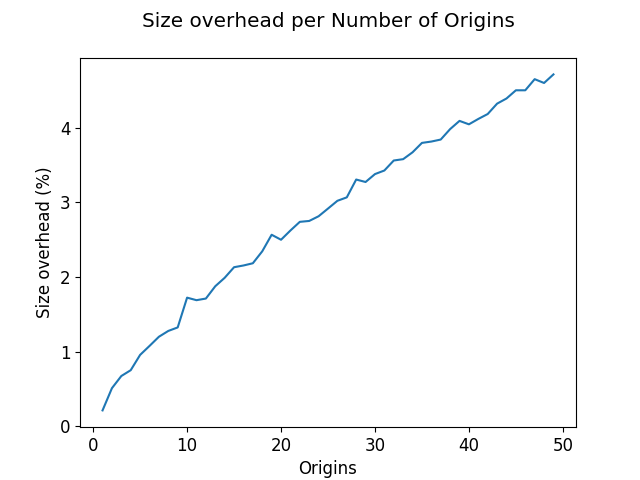
\includegraphics[width=0.48\textwidth]{experiments/ctx_performance/origins.png}
        \caption{Origins}
        \label{fig:origin_ctx}
    \end{figure}

As Figure \ref{fig:origin_ctx} shows, the size overhead when 1 origin is used is
less than 0.5\% and about 4.7\% when 50 origins are used. This means that in our
worst-case scenario, the compressed CTX-protected response is 1.047 times the
unprotected compressed response.

The second parameter, the total response size, reflects the scalability of CTX.
In this case, we use 50 origins and consider 1\% of the total response to be
secret, equally distributed in all origins. The length of the response page
ranges from 13KB to 650KB.

Our experiments show that the increase in bytes that CTX adds is not
proportional to the increase of the total response size. This results in a
significant overhead for small web pages, which becomes less observable as the
web page grows larger.

    \begin{figure}[thpb]
        \centering
            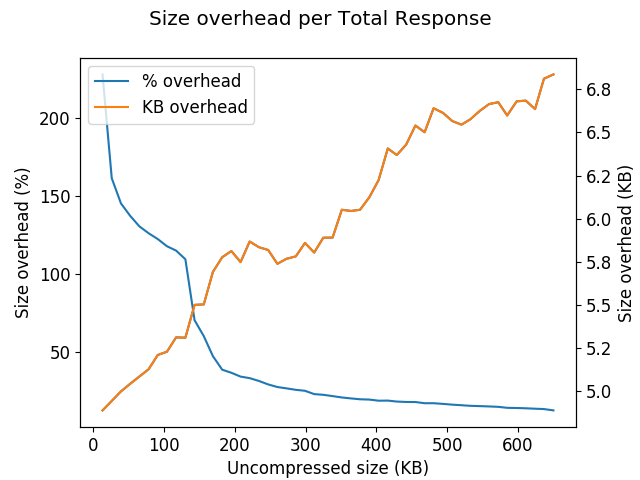
\includegraphics[width=0.48\textwidth]{experiments/ctx_performance/total_response.png}
        \caption{Total response}
        \label{fig:total_response_ctx}
    \end{figure}

Figure \ref{fig:total_response_ctx} depicts the results of this experiment. A
13KB web page suffers a 5KB CTX overhead, which corresponds to a 228\% increase
in compressed response. On the other hand, CTX will add only 7KB for a 650KB web
page, which results in a 12\% increase. In comparison, the overhead for
disabling compression entirely would range from 500\% to 1000\% for the tested
web pages, while, for this last case of the 650KB web page, the secret masking
method previously suggested in the literature adds a 21\% overhead.

The third parameter is the total amount of secrets in the response. We now use
a 650KB web page with 50 origins. The secrets amount from 1\% up to 50\% of the
web page, the rest being static data, and are evenly distributed across origins.

    \begin{figure}[thpb]
        \centering
            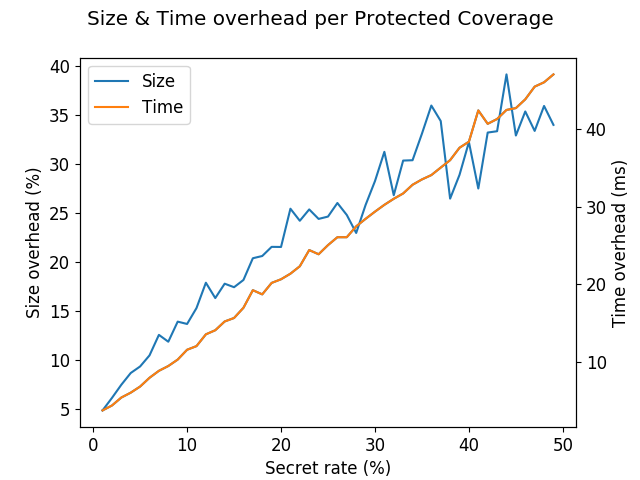
\includegraphics[width=0.48\textwidth]{experiments/ctx_performance/response_secrets.png}
        \caption{Response secrets}
        \label{fig:response_secrets_ctx}
    \end{figure}

Figure \ref{fig:response_secrets_ctx} shows the results of this experiment. We
find that protecting 1\% of this web page results in less than 5\% size
overhead, whereas protecting 50\% of the page results in 35\% overhead. The time
increase is also noteworthy in this case, where CTX adds 10ms of execution time
for 10\% secrets in the web page and 47ms for 50\% secrets.

In comparison, disabling compression would result in 976.8\% load overhead
and a network transmission time overhead that, depending on the client's and the
server's network, may be several seconds.

\subsection{Security of CTX}

We now move on to describe a series of lemmas that show certain conditions
which allow for provable reflection security. This direction supports
the design decisions for CTX. While we do not formally prove the security of
CTX, we argue that it is empirically similar to provably secure schemes.

We start by providing the full proof for a simple construction. We then move on
to provide proof sketches for consecutively more complicated constructions,
until we reach a construction which we argue is very similar to CTX.

In the lemmas below, we use the shorthand $E$ to refer to the encryption
function of an encryption schema $(Gen, E, D)$. We talk about the reflection
security of various schemes which are defined by their output. For example,
when we say that $E(s) || E(r)$ is reflection secure, we mean that the function
defined as $\widetilde{E}(s, r) = E(s) || E(r)$ is reflection secure.

Complete proofs of all lemmas can be found in Appendix A.

\begin{lemma}[Reflection-independent security]
    Let $E$ be a length-preserving semantically secure encryption schema and
    $Com$ be any function. Then $E(s)$ is reflection secure.
\end{lemma}

\begin{lemma}
    Under the above assumptions, $E(s) || r$ is reflection secure.
\end{lemma}

\begin{lemma}
    Under the above assumptions and letting $Com$ be a deterministic
    efficiently computable function, $E(s)$ $||$ $Com(r)$ is reflection secure.
\end{lemma}

\begin{lemma}
    Under the above assumptions and additionally requiring that $Com$ is a
    bijection which is also efficiently reversible, $E(Com(s))$ is reflection secure.
\end{lemma}

\begin{lemma}
    Under the above assumptions, $E(Com(s)) || r)$, \break$E(Com(s)) || E(r))$, and
    $E(Com(s)) || E(Com(r))$ are all reflection secure.
\end{lemma}

\begin{lemma}
    Under the above assumptions, $E(s || r)$ is reflection secure.
\end{lemma}

\begin{lemma}
    Under the above assumptions, $E(Com(s)$ $||$ $Com(r))$ is reflection secure.
\end{lemma}

We are now ready to argue for the security of CTX. Let the function $ctx(s)$
denote the substitution cipher applied on $s$ using a uniformly random alphabet
permutation. We make the simplifying assumption that $ctx(s)$ only contains the
ciphertext where the substitution cipher has been applied and that the exact
permutation required to reverse the substitution cipher is sent through a
separate secure channel.

Under the assumption that \[|Com(s) || Com(r)| = |Com(ctx(s) || ctx(r))|\] we
see that the semantically secure function $E$ will not allow distinguishing
between the two distributions $Com(s) || Com(r)$ and $Com(ctx(s) || ctx(r))$.

Clearly, these two lengths will not be equal for adversarial compression
functions Com. However, we argue that they are almost equal for realistic
instances of compression functions.

In order to back our claim, we perform the following experiment. We choose a
fixed secret $s$, 100 characters long. We then choose the reflections $r_i,
i\in[0, 50]$, where $|r_i| = 50 + i*20$. For each $r_i$ we calculate the
length of separate compression using gzip $|gzip(s)||gzip(r_i)|$ and the length
of the compressed CTX'ed secret and reflection $|gzip(ctx(s), ctx(r_i))|$, where $s$
and $r_i$ belong to different origins.

The results are shown in figure \ref{fig:defense_experiment}. It can be seen
that the outputs of these two methods are linearly correlated, with the
Pearson correlation coefficient of the two variables being 0.998712.

    \begin{figure}[thpb]
        \centering
            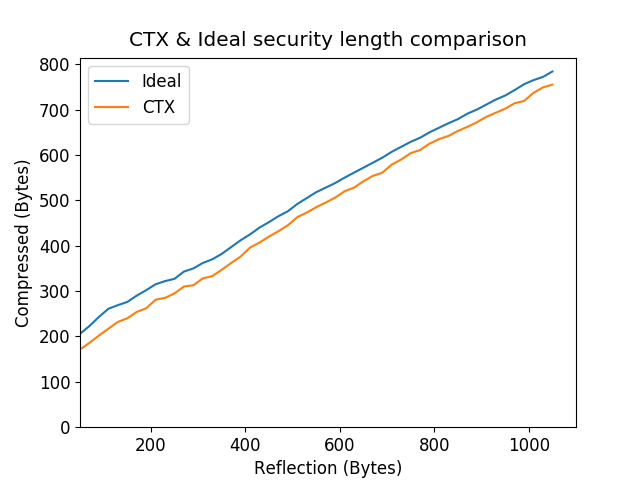
\includegraphics[width=0.48\textwidth]{experiments/ctx_idealness/ctx_experiment.png}
        \caption{CTX/Theoretical security comparison}
        \label{fig:defense_experiment}
    \end{figure}
